\documentclass[oneside]{book}
\usepackage[utf8]{inputenc}
\usepackage{amsmath}
\usepackage{amssymb}
\usepackage{amsfonts}
\usepackage{tikz,pgfplots}
\pgfplotsset{compat=1.18}
\usepackage{geometry}
\geometry{
  bottom=15mm
}
\usepackage{textcomp, gensymb}
\usepackage{hyperref}
\hypersetup{
    colorlinks=true,
    linkcolor=blue,
    filecolor=magenta,      
    urlcolor=cyan,
    }
\AddToHook{shipout/background}{%
\put (0in,-\paperheight){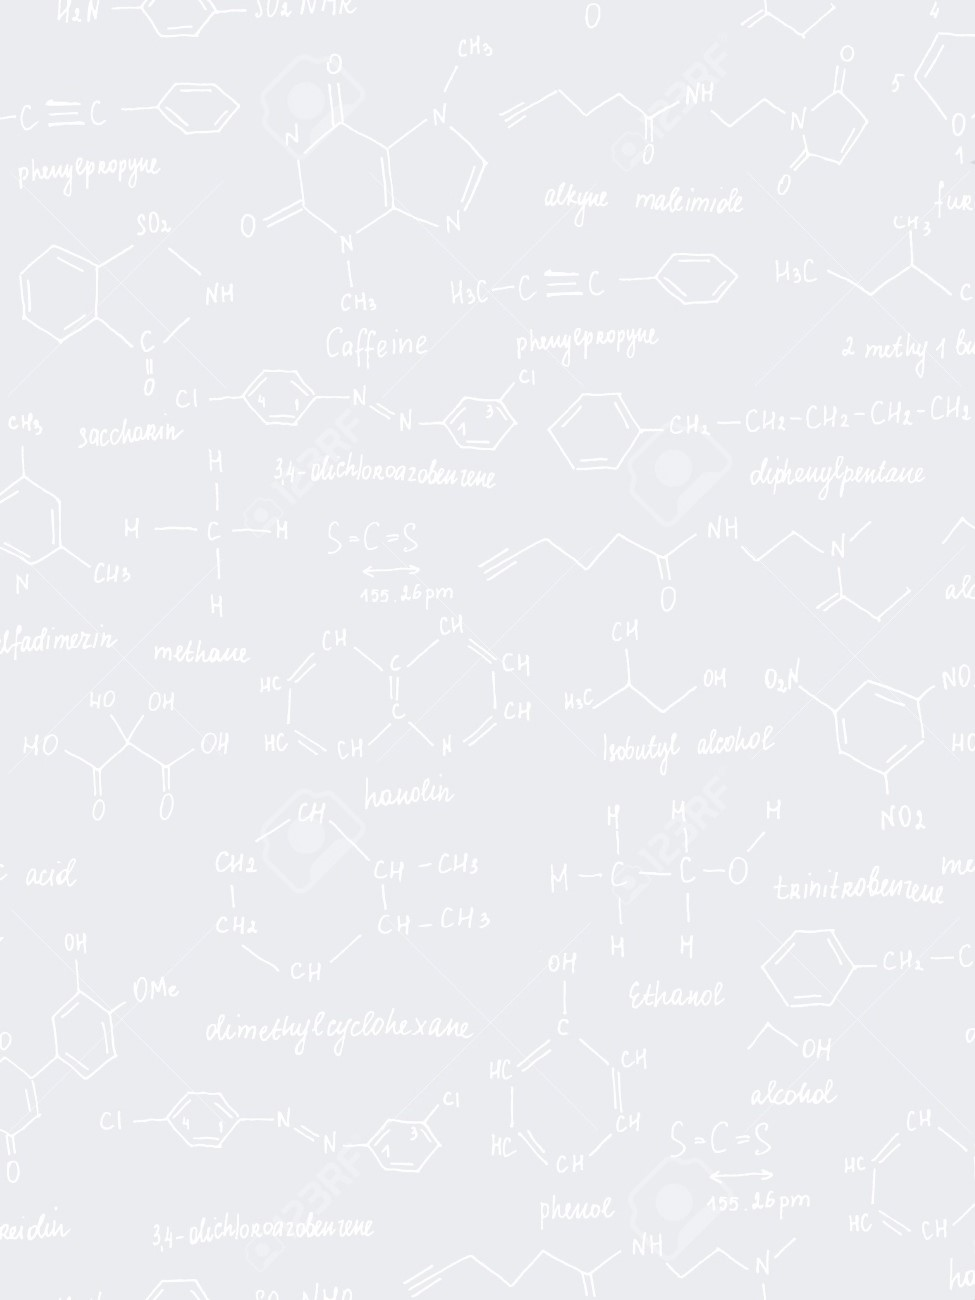
\includegraphics[width=\paperwidth,height=\paperheight]{C.jpeg}}%
}
\usepackage{graphicx}
\graphicspath{ {./images/} }

\usepackage[pagestyles]{titlesec}
\titleformat{\chapter}[display]   
{\normalfont\huge\bfseries}{\chaptertitlename\ \thechapter}{20pt}{\Huge}   
\titlespacing*{\chapter}{0pt}{-50pt}{40pt}
\titleformat{\chapter}[display]{\normalfont\bfseries}{}{0pt}{\Huge}
\newpagestyle{mystyle}
{\sethead[\thepage][][\chaptertitle]{}{}{\thepage}}
\pagestyle{headings}

\begin{document}

\begin{tikzpicture}[font=\sffamily,remember picture,overlay]
    \path (current page.north west) node[below right,fill={rgb:orange,0.55;yellow,2.5;pink,1.5},minimum 
    width=\paperwidth,minimum height=3cm](box){};
    
    \path (box.west) node[right=5cm,align=center] %<distance can be changed to suit
    {{\fontsize{45pt}{65pt}\color{white}\textbf{Chemistry Learning Points}}\\[2mm]
    {\fontsize{30pt}{20pt}\color{white}Grass}\\[2mm]
    {\fontsize{10pt}{10pt}\color{white}August 2022}};
    
\end{tikzpicture}

\begin{enumerate}
    \item \emph{\textbf{The Air is made of Air:}} Read the question carefully!
    \item Displacement: \textbf{Ions} are displaced! Not elements or compounds.\\ \footnotesize (So say like \(I^{-}\) is displaced, not \( I_2 \) ) \normalsize
    \item Safer to just quote the data if given; i.e. 
    \footnotesize As the bond length decreases from \emph{0.092 to 0.16nm}, the bond energy increases from \emph{614 \( kJ/mol \) to 299 \( kJ/mol \)} \normalsize
    \item Mention the \textbf{specfic} reactants involved for the energy released in bond forming and energy absorbed in bond breaking.\\
    (As well as the no. of moles for each reactant and product involved in the reaction if given.)
    \item Aqueous Bromine, \( Br_{2_{(aq)}} \), is reddish-brown. While aqueous iodine, \( I_{2_{(aq)}} \), is brown. 
    \item Why does metal \(\Gamma\) remain shiny after being exposed to \(\Sigma\) substance?\\
     \footnotesize (Esp. for \(Al\) and stainless steel / \(Cr\) ) \normalsize\\
    A layer of unreactive \(\Gamma\) oxide costs the \(\Gamma\) metal, protecting it from corrosion / reacting with \(\Sigma\) substance.
    \item Rmb that observation is what what you can see, smell, etc.\\ 
    \footnotesize So like write \emph{"colorless, odorless gas would be evolved"} instead of \emph{"oygen gas is evolved"} \normalsize
    \item Noble gases naturally exists with \emph{stable electronic structure}, where their \emph{valence shell is completely filled}. Thus they are \emph{unreactive}. Hence, they \textbf{will not be involved in chemical bonding.}
    \item Why is \( CO_2 \) not a gas harmful to human health?\\
    Carbon dioxide is a relatively harmless gas, which is also produced naturally by the human body during respiration.
    \item Why is a black smoke seen after burning hydrocarbons?\\
    \footnotesize It is the carbon soot formed by the \textbf{incomplete} combustion of the hydrocarbons. \normalsize
    \item Checking for presence of salts in an aqueous solution:\\
    Carry out evaporation to dryness. If dissolved salts are present, a residue / solid will be left behind.\\
    \footnotesize (But if the qns ask for checking the purity of the aqueous solution, then can just use the normal method of seeing if it boils over a range of temperatures / only begin boiling at a higher temperature than expected) \normalsize 
    \item The catalyst for the decomposition of hydrogen peroxide (\(H_2O_2\)) is maganese (IV) oxide
    \item Acidified potassium dichromate (Oxidising Agent): Changes from orange to green (Test for reducing agent) \small
    \item \begin{center}
        \begin{tabular}{ |c|c| }  
            \hline
            \color{blue} Oxidising Agents & \color{blue} Reducing Agents\\
            \hline
            Bromine \(Br_2\) & Carbon \(C\)\\
            \hline
            Chlorine \(Cl_2\) & Carbon Monoxide \(CO\)\\
            \hline
            Concentrated Sulfuric Acid \(H_2SO_4\) & Hydrogen \(H_2\)\\
            \hline
            Nitric Acid \(NO\) & Hydrogen Sulfide \(H_2S\)\\
            \hline
            Oxygen \(O_2\) & Metals\\
            \hline
            Potassium Maganate (VII) \(KMnO_4\) & Potassium Iodide \(KI\)\\
            \hline
            Potassium Dichromate (VI) \(K_2Cr_2O_7\) & Sulfur Dioxide \(SO_2\)\\
            \hline
        \end{tabular}
        \end{center}
        \item
    \begin{center}
        \begin{tabular}{ |c|c|c| }  
            \hline
            \color{blue} Compound & \color{blue} Chemical formula & \color{blue} Colour\\
            \hline
            Chromium (III) Chloride & \( CrCl_3 \) & Green\\
            \hline
            Iron (II) Sulfate & \(FeSO_4\) & Pale Green\\
            \hline
            Magnanese (IV) Oxide & \(MnO_2\) & Black\\
            \hline
            Copper (I) oxide & \(Cu_2O\) & Red\\
            \hline
            Iron (III) Chloride & \(FeCl_3\) & Yellow\\
            \hline
            Potassium Maganate (VII) & \(KMnO_4\) & Purple\\
            \hline
            Copper (II) Oxide & \(CuO\) & Black\\
            \hline
        \end{tabular}
        \end{center}
\end{enumerate}





\end{document}